This section serves as a detailed description of how we fully assemble the membrane-in-the-middle setup. It is a long and sometimes tedious procedure. Most of the procedure is constructed from educated guesses, while a procedure like fixing the membrane versus flat mirror tilt is pure luck, i.e. trial and error.

\subsection{Cleaning}
To achieve good vacuum the sample holder including screws, springs and membrane spacers is cleaned in high purity acetone inside an ultra-sonic bath for roughly 20 minutes. After the ultra-sonic bath the parts are pulled out of the acetone, in as clean conditions as possible inside a lab/fume hood, and cleaned with ``ultrapure\footnote{Millipore}" water to get rid of any residual acetone and small impurities. The parts are then put aside to dry on the inside of a piece of aluminum foil. When dried the parts are ready to used inside our cryostat.

We depend a lot on our mirrors to have low losses and they fulfill this task. But mirrors can also become dusty or dirty from small broken silicon parts of the spacers. The tiny silicon impurities on the mirrors can occur when tightening the screws between middle and bottom part of the sample holder because it sometimes happens that the membrane stack is slightly misplaced and silicon pieces are broken of the stack. We clean the mirrors with a polymer\footnote{First Contact. Nice videos showing this procedure can be found on \url{https://www.youtube.com/watch?v=YWp8k8s8aeM}.} evenly distributed on the coated mirror surface. The polymer dries out and can be pulled of with a suitable adhesive tape. The mirrors are then checked under a microscope before being put into use.

It is important to use and wear for example clean plastic tweezers, rubber gloves, hairnet and face mask, while cleaning the individual parts for minimizing contamination as much as possible.

\subsection{Back reflection}
We tightly screw the bottom sample holder piece into the cold finger inside the cryostat, and place a copper wave spring with the flat mirror on top of it inside the hole in the sample holder. The flat mirror is now resting on the spring. We then shine laser light on to the mirror and try to maximize back reflection through the fiber. Backreflection coupled in to the fiber is maximum, when you mode-match, i.e have the waist on the flat mirror. It allows for a good initial parameter for mode matching.

\subsection{Membrane tilt}
The next step is to carefully assemble the spacer-membrane-spacer stack and place it on top of the flat mirror. The middle sampler holder part is put onto the stack and screwed into place compressing the spring and making a tight and hopefully parallel fit between membrane surface and mirror surface. The membrane and the mirror now make up an unstable low finesse cavity, due to the relative low reflectivity coefficient of the silicon nitride membrane. It is this cavity that enables us via scanning the fiber output coupler in the same plane as the combined membrane-mirror plane to observe cavity resonance fringes. The tilt angle can be extrapolated from number of fringes showing up on the oscilloscope. Each fringe corresponds to another half wavelength fitting into the cavity and if we note down the range of the scan we also know the angle from simple geometry. The goal is to eliminate fringes by trial and error, by pushing unscrewing the middle piece a little bit and then screwing it back in again. A successful attempt is shown in figure \ref{fig:mem_tilt}.

\begin{figure}[H]
\centering
    \begin{subfigure}[b]{0.49\textwidth}
    \centering
    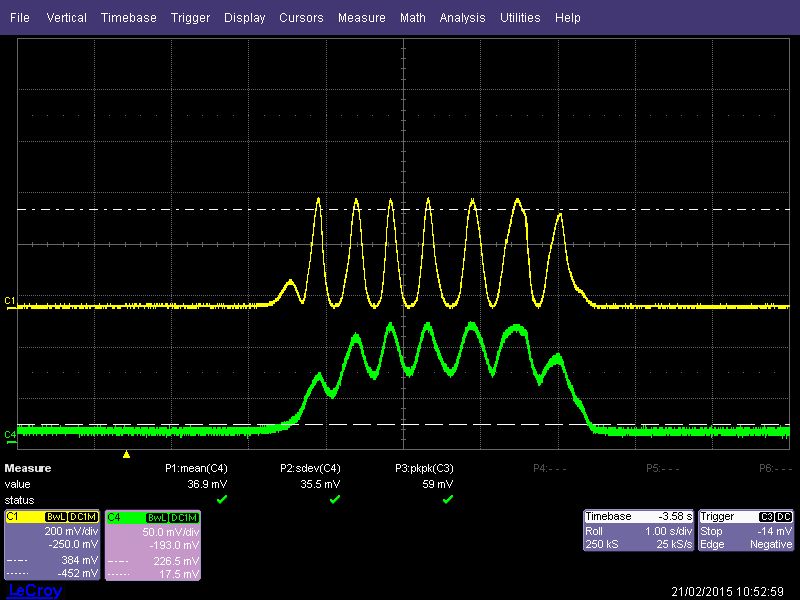
\includegraphics[width=\textwidth]{yscan.png}
    \caption{}
    \label{fig:yscan}
    \end{subfigure}
    \hfil
    \begin{subfigure}[b]{0.49\textwidth}
    \centering
    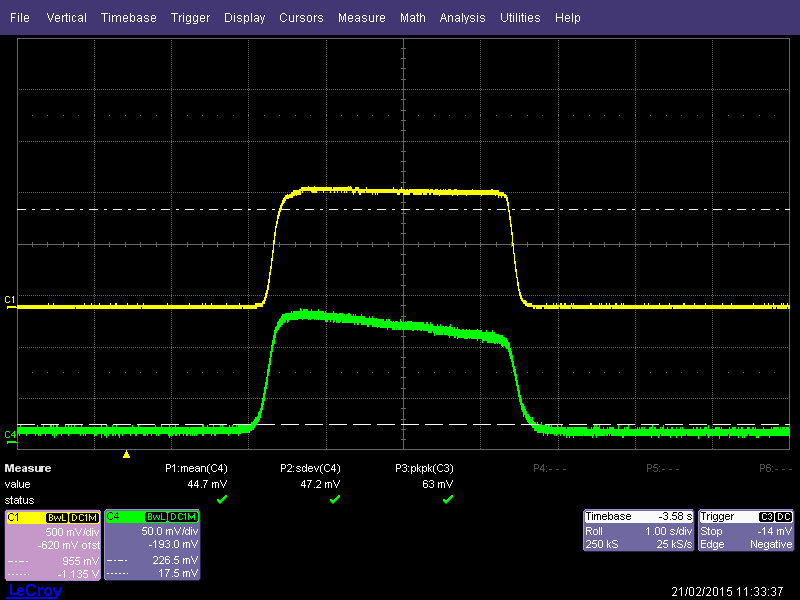
\includegraphics[width=\textwidth]{yscan_after.png}
    \caption{}
    \label{fig:yscan_after}
    \end{subfigure}
\caption{Screenshots of the oscilloscope display showing transmission and reflection curves as the laser beam is moved across the membrane. (a) Before fixing the tilt and (b) after fixing the tilt.}
\label{fig:mem_tilt}
\end{figure}

\subsection{Cavity alignment}
When the tilt is minimized we put in the top mirror and place a spring on top of it before enclosing it with the top sample holder piece. The screws are not screwed all the way in because we need to push around the top curved mirror to obtain a cavity. This is the so called ``pinhead procedure". It can be advantageous to go a wavelength with a relative low finesse to make life a bit easier, because lower finesse cavities have broader resonance and are therefore more likely to be spotted while scanning the laser wavelength. This trick is general when assembling cavities.

When a cavity has been realized we move to a high finesse wavelength (\SI{852}{\nano\meter}) and scan the wavelength until we see the transverse mode $TEM_{(00)}$ on the camera, see figure \ref{fig:beam_place}. We then maximize the transmission of this transverse mode, by scanning the laser frequency fast across the cavity resonance and optimizing the cavity response detected on the transmission detector.

\subsection{Illumination of membrane}
We use four LED's placed tightly together in a circle with a hole in the middle, allowing for the laser beam to pass through and put it in the beam path, just before the cavity, we can illuminate the membrane and roughly estimate our beam position on the membrane mode as shown in figure \ref{fig:beam_place}.

\begin{figure}[H]
\centering
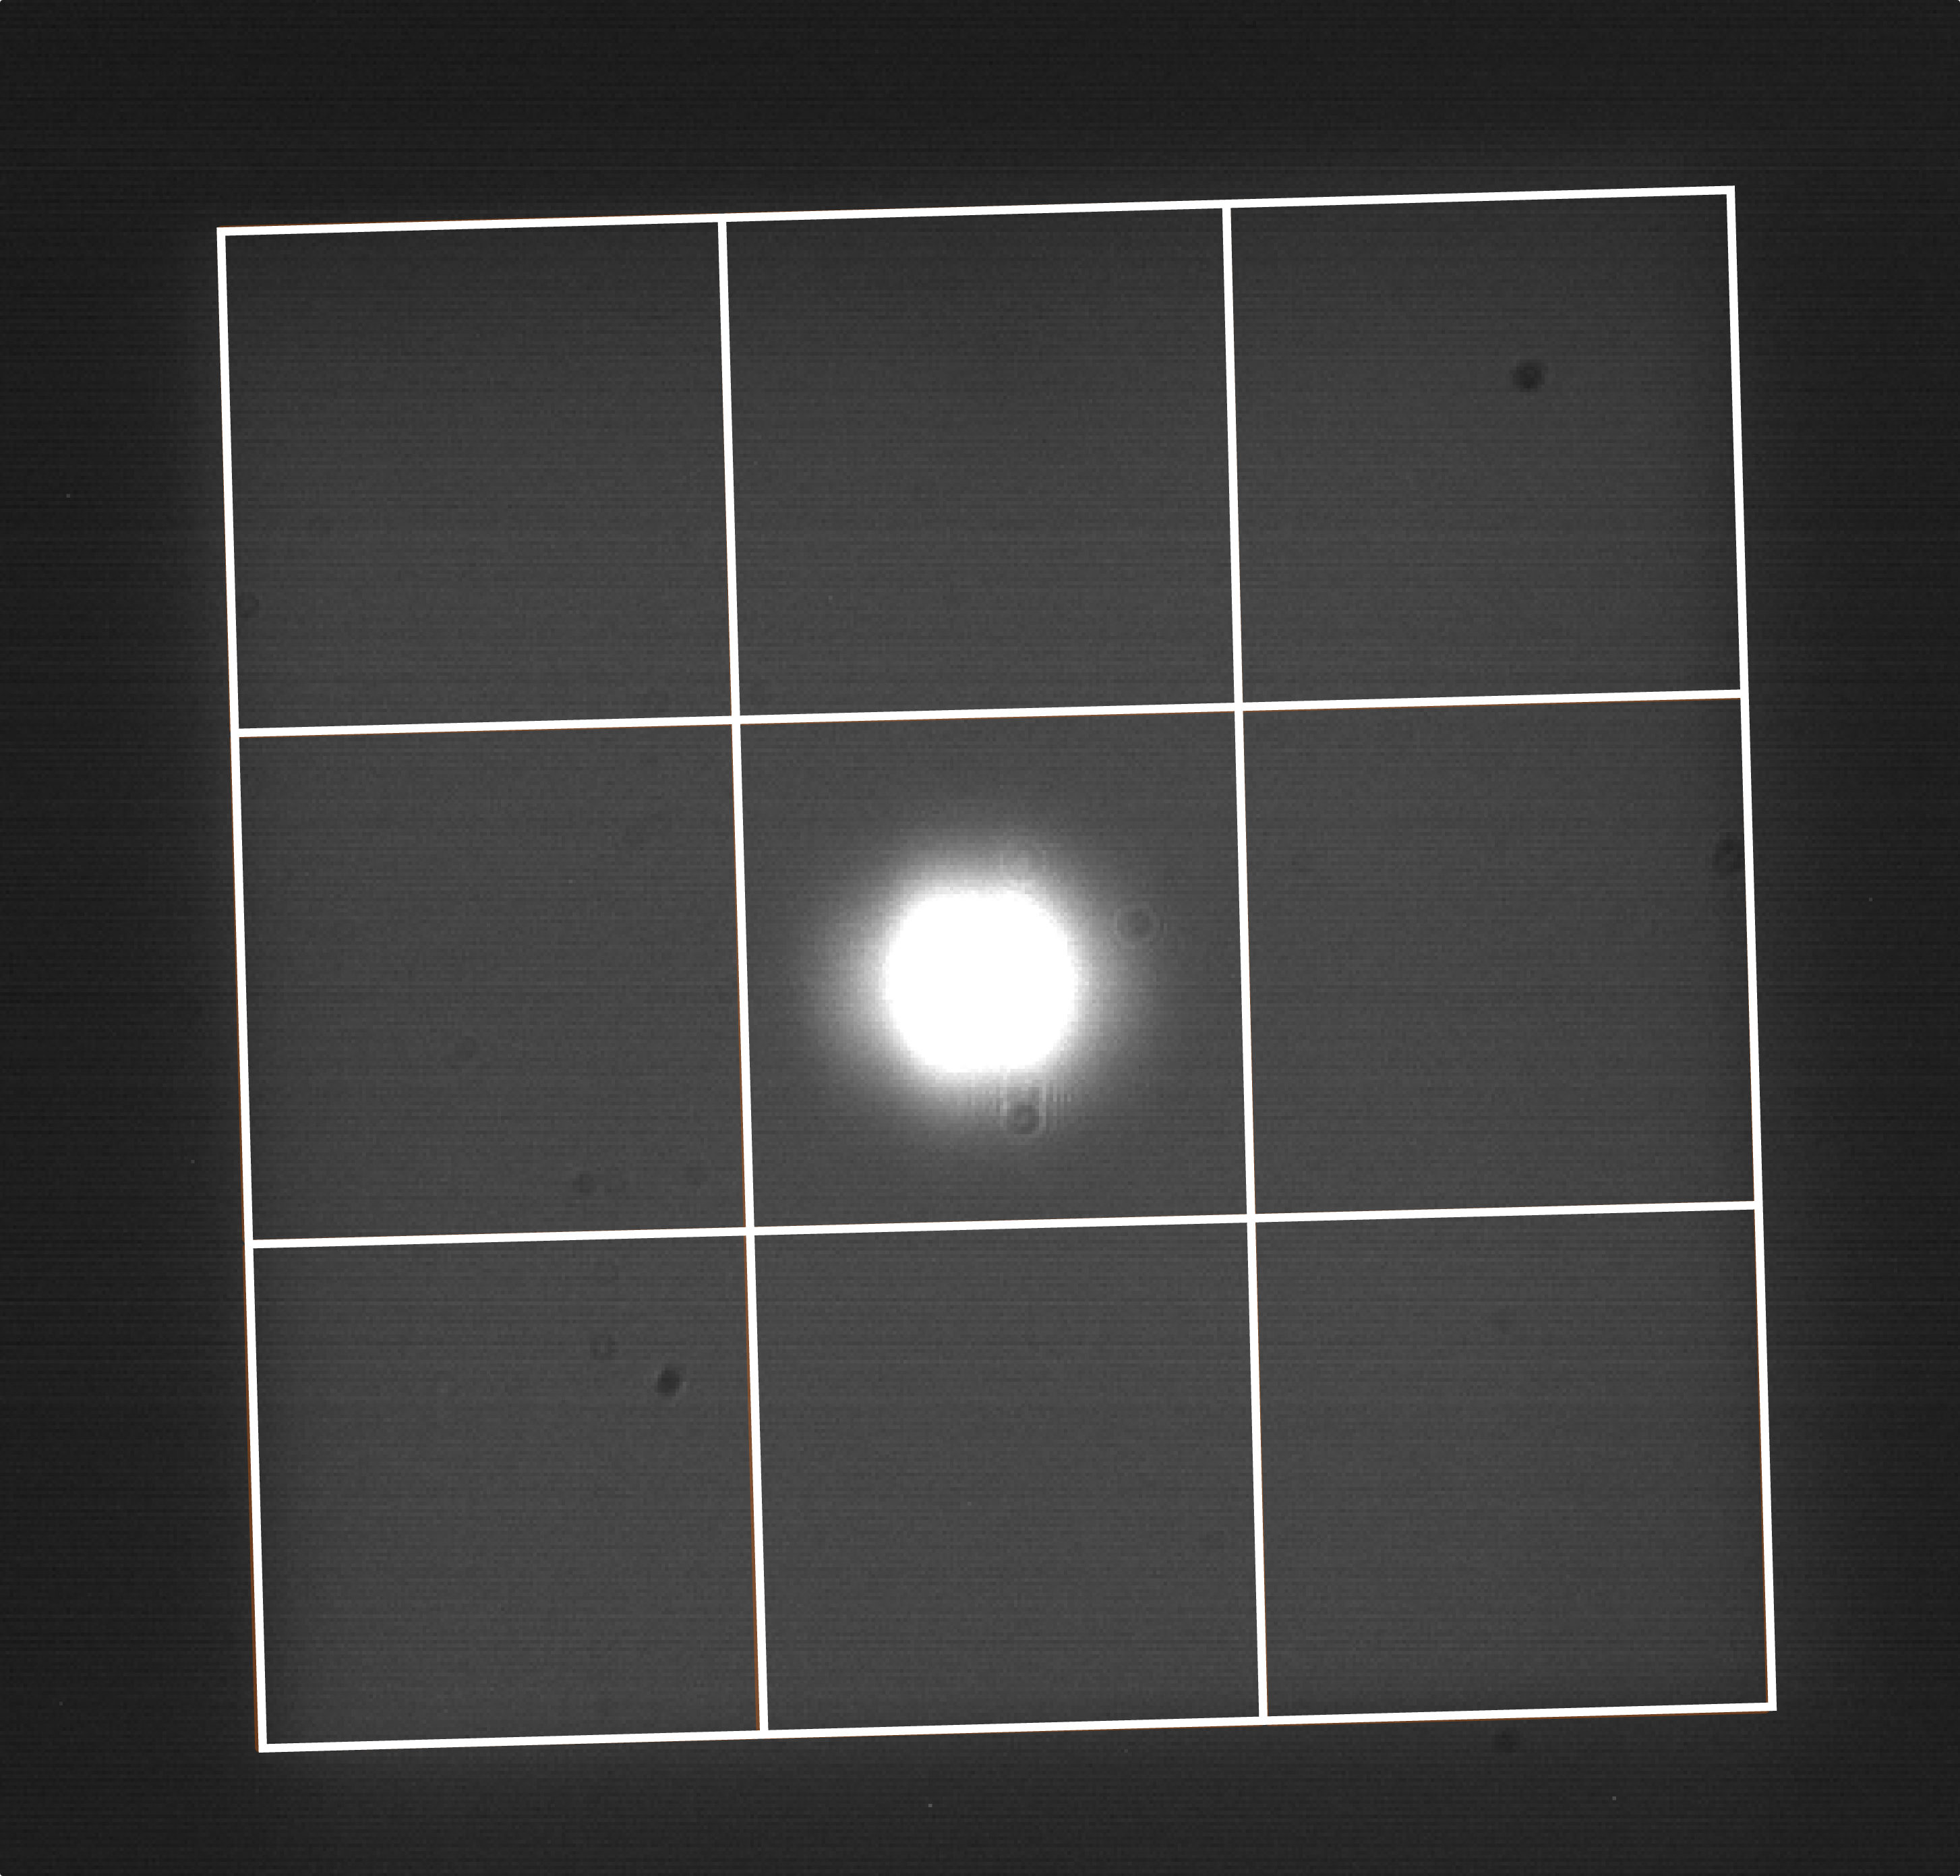
\includegraphics[scale=0.5]{membraneGrid.png}
\caption{Screenshot of the camera picture showing the illuminated membrane and the $TEM_{(00)}$ mode. The orange squares refers to the outline of the mechanical (3,3)-mode nodes.}
\label{fig:beam_place}
\end{figure}

A large overlap between the mechanical modes antinode and laser spot ensures a better coupling between the optical and mechanical degree of freedom.